\chapter{Взаимодействие волноводов}
\label{coupling}
\section{Поле цилиндрического волновода}
Как уже упоминалось ранее, цилиндрический волновод имеет следующее распределение поля (формула \ref{cylinder_bessel}):
$$
	H_z = H_0 J_v (\frac{ur}{a}).
$$
Для основной моды $v = 0$, а распределение можно считать распределением Гаусса. Сначала, учитывая  симметриею цилиндрического волновода рассмотрим проекцию поля на плоскость осевого сечения $xz$. В этом случае продольная составляющая будет зависеть только от $x$ и распределение примет вид:
\begin{equation}
  \label{gauss}
  E(x)=\frac{1}{\sigma\sqrt{2\pi}}\exp\left(-\frac{x^2}{2\sigma^2}\right)
\end{equation}
Формула описывает нормальное распределение с вершиной в точке $x=0$.
Здесь $\sigma = 1,1a$ - радиус моды, $a$ - радиус волновода. Соотношение соблюдается на длине волны, близкой к длине отсечки: $1 < \frac{\lambda}{\lambda_c} < 1.5$
Для сравнения, на рисунке \ref{diameter} показаны распределения поля волноводов разной толщины.

\begin{figure}[h!]
	\begin{minipage}[h]{0.49\linewidth}
		\center{\includegraphics[width=1\linewidth]{img/field_distribution.png} \\ а)}
	\end{minipage}
	\hfill
	\begin{minipage}[h]{0.49\linewidth}
		\center{\includegraphics[width=1\linewidth]{img/field_distribution2.png} \\ б)}
	\end{minipage}
	\caption{Распределение поля в волноводах с разным радиусом моды: \mbox{а) 7~мкм, б) 4~мкм}}
	\label{diameter}
\end{figure}

Целью данной работы является рассмотрение эффективности передачи энергии при соединении волноводов. Опишем эту зависимость теоретически.

Коэффициент передачи энергии определяется отношением скалярных квадратов мощности связанной волны к мощности входной волны \cite{lefevre}.

\begin{equation}
	\label{coupling_full}
	C = \frac{\left[\int\limits_{-\infty}^{\infty}E_{in}(x)e_{f0}^*(x) \,dx\right]^2}
	{\int\limits_{-\infty}^{\infty}e_{f0}(x)e_{f0}^*(x) \,dx
	 \int\limits_{-\infty}^{\infty}E_{in}(x)E_{in}^*(x) \,dx}
\end{equation}

\begin{figure}[h!]
	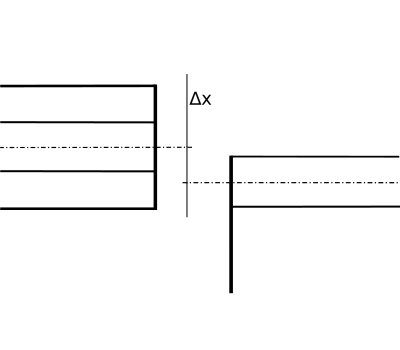
\includegraphics[width=.5\textwidth]{img/transverse_movement.pdf}
	\caption{Поперечное смещение волноводов}
	\label{transverse_movement}
\end{figure}

Рассмотрим изменение взаимного расположения полей в зависимости от поперечного смещения волноводов. В этом случае фаза не изменяется, а значит комплексная часть распределения равна нулю, а формула примет вид:

\begin{equation}
	\label{coupling}
	C = \frac{\left[\int\limits_{-\infty}^{\infty}E_{in}(x)e_{f0}(x) \,dx\right]^2}
	{\int\limits_{-\infty}^{\infty}e_{f0}(x)^2 \,dx
	 \int\limits_{-\infty}^{\infty}E_{in}(x)^2 \,dx}
\end{equation}

Это выражение называется интегралом перекрытия  и показывает, какая часть энергии перейдет в возбуждение моды во втором волноводе. 

Рассмотрим поперечное смещение волноводов. При этом их поля также сместятся относительно друг друга и будут перекрываться не полностью.

\begin{figure}[h!]
	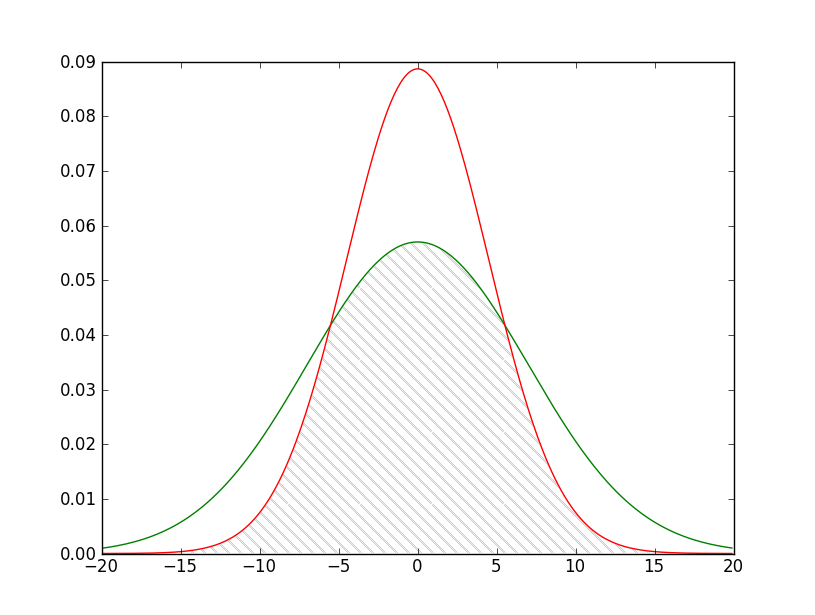
\includegraphics[width=.5\textwidth]{img/intersection.png}
	\caption{Распределение полей при поперечном смещении}
\end{figure}

В показанном выше случае, поле возбуждаемой моды имеет максимум при $x=0$, а поле в входном волноводе имеет максимум в точке $x=4$. Из-за этого несоответствия интенсивность света выходном волноводе уменьшается. Очевидно что коэффициент передачи, то есть отношение интенсивности в выходном волноводе ко входному, максимален и равен 1 при условии $E_{in} \equiv e_{f0}$.

\section{Поле волноводов в пространстве}

Выше рассматривалась проекция распределения поля на плоскость. В пространстве гауссово распределение зависит от двух координат и равно:
\begin{equation}
  \label{gauss3d}
  E(x,y)=\frac{1}{2\pi\sigma_1\sigma_2}\exp\left(-\frac{x^2}{2\sigma_1^2}-\frac{y^2}{2\sigma_2^2}\right)
\end{equation}
где $\sigma_1$ и $\sigma_2$ - радиус моды по осям $x$ и $y$ соответственно. График этого уравнения выглядит представлен на рисунке \ref{gauss3dPlot}.
\begin{figure}[h!]
	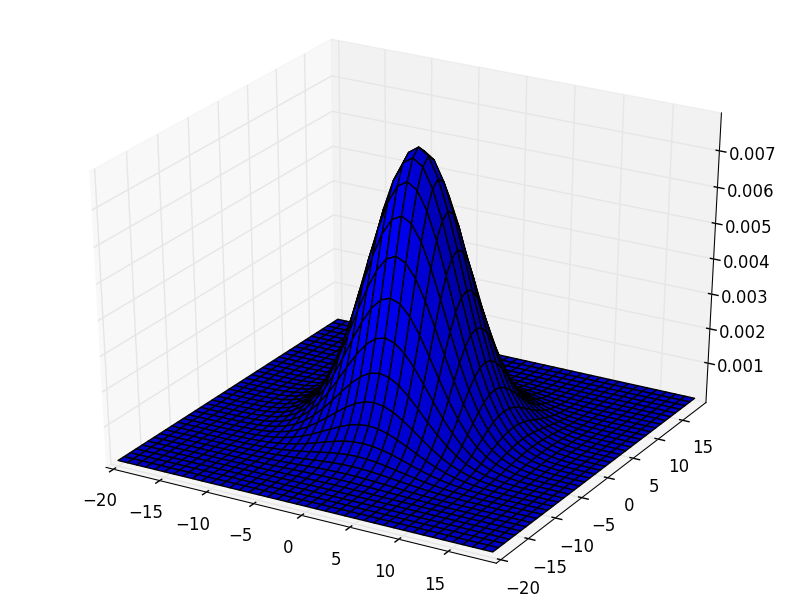
\includegraphics[width=0.5\textwidth]{img/gauss3d.png}
	\caption{Распределение Гаусса в пространстве}
	\label{gauss3dPlot}
\end{figure}

Интеграл перекрытия также будет зависеть от двух переменных и примет вид:

\begin{equation}
	\label{coupling}
	C = \frac{\left[\iint\limits_{-\infty}^{\infty}E_{in}(x,y)e_{f0}(x,y) \,dxdy\right]^2}
	{\iint\limits_{-\infty}^{\infty}e_{f0}(x,y)^2 \,dxdy
	 \iint\limits_{-\infty}^{\infty}E_{in}(x,y)^2 \,dxdy}
\end{equation}
